% Options for packages loaded elsewhere
\PassOptionsToPackage{unicode}{hyperref}
\PassOptionsToPackage{hyphens}{url}
%
\documentclass[
]{article}
\usepackage{amsmath,amssymb}
\usepackage{lmodern}
\usepackage{iftex}
\ifPDFTeX
  \usepackage[T1]{fontenc}
  \usepackage[utf8]{inputenc}
  \usepackage{textcomp} % provide euro and other symbols
\else % if luatex or xetex
  \usepackage{unicode-math}
  \defaultfontfeatures{Scale=MatchLowercase}
  \defaultfontfeatures[\rmfamily]{Ligatures=TeX,Scale=1}
\fi
% Use upquote if available, for straight quotes in verbatim environments
\IfFileExists{upquote.sty}{\usepackage{upquote}}{}
\IfFileExists{microtype.sty}{% use microtype if available
  \usepackage[]{microtype}
  \UseMicrotypeSet[protrusion]{basicmath} % disable protrusion for tt fonts
}{}
\makeatletter
\@ifundefined{KOMAClassName}{% if non-KOMA class
  \IfFileExists{parskip.sty}{%
    \usepackage{parskip}
  }{% else
    \setlength{\parindent}{0pt}
    \setlength{\parskip}{6pt plus 2pt minus 1pt}}
}{% if KOMA class
  \KOMAoptions{parskip=half}}
\makeatother
\usepackage{xcolor}
\usepackage[margin=1in]{geometry}
\usepackage{graphicx}
\makeatletter
\def\maxwidth{\ifdim\Gin@nat@width>\linewidth\linewidth\else\Gin@nat@width\fi}
\def\maxheight{\ifdim\Gin@nat@height>\textheight\textheight\else\Gin@nat@height\fi}
\makeatother
% Scale images if necessary, so that they will not overflow the page
% margins by default, and it is still possible to overwrite the defaults
% using explicit options in \includegraphics[width, height, ...]{}
\setkeys{Gin}{width=\maxwidth,height=\maxheight,keepaspectratio}
% Set default figure placement to htbp
\makeatletter
\def\fps@figure{htbp}
\makeatother
\setlength{\emergencystretch}{3em} % prevent overfull lines
\providecommand{\tightlist}{%
  \setlength{\itemsep}{0pt}\setlength{\parskip}{0pt}}
\setcounter{secnumdepth}{-\maxdimen} % remove section numbering
\ifLuaTeX
  \usepackage{selnolig}  % disable illegal ligatures
\fi
\IfFileExists{bookmark.sty}{\usepackage{bookmark}}{\usepackage{hyperref}}
\IfFileExists{xurl.sty}{\usepackage{xurl}}{} % add URL line breaks if available
\urlstyle{same} % disable monospaced font for URLs
\hypersetup{
  pdftitle={TMA4268 Statistical Learning},
  pdfauthor={Daesoo Lee, Emma Skarstein, Kenneth Aase, Stefanie Muff; Department of Mathematical Sciences, NTNU},
  hidelinks,
  pdfcreator={LaTeX via pandoc}}

\title{TMA4268 Statistical Learning}
\usepackage{etoolbox}
\makeatletter
\providecommand{\subtitle}[1]{% add subtitle to \maketitle
  \apptocmd{\@title}{\par {\large #1 \par}}{}{}
}
\makeatother
\subtitle{Module 6: Recommended exercises}
\author{Daesoo Lee, Emma Skarstein, Kenneth Aase, Stefanie
Muff \and Department of Mathematical Sciences, NTNU}
\date{Spring 2023}

\begin{document}
\maketitle

{
\setcounter{tocdepth}{2}
\tableofcontents
}
\hypertarget{recommended-exercise-1}{%
\section{Recommended exercise 1}\label{recommended-exercise-1}}

\begin{enumerate}
\def\labelenumi{\arabic{enumi}.}
\tightlist
\item
  Show that the least square estimator of a standard linear model is
  given by
  \[ \hat{\boldsymbol \beta} =(\boldsymbol X^T \boldsymbol X)^{-1} \boldsymbol X^T \boldsymbol Y\]
\item
  Show that the maximum likelihood estimator is equal to the least
  square estimator for the standard linear model.
\end{enumerate}

\hypertarget{recommended-exercise-2}{%
\section{Recommended exercise 2}\label{recommended-exercise-2}}

Write R code to create a similar representation of the Credit data
figure shown below.

\begin{figure}
\centering
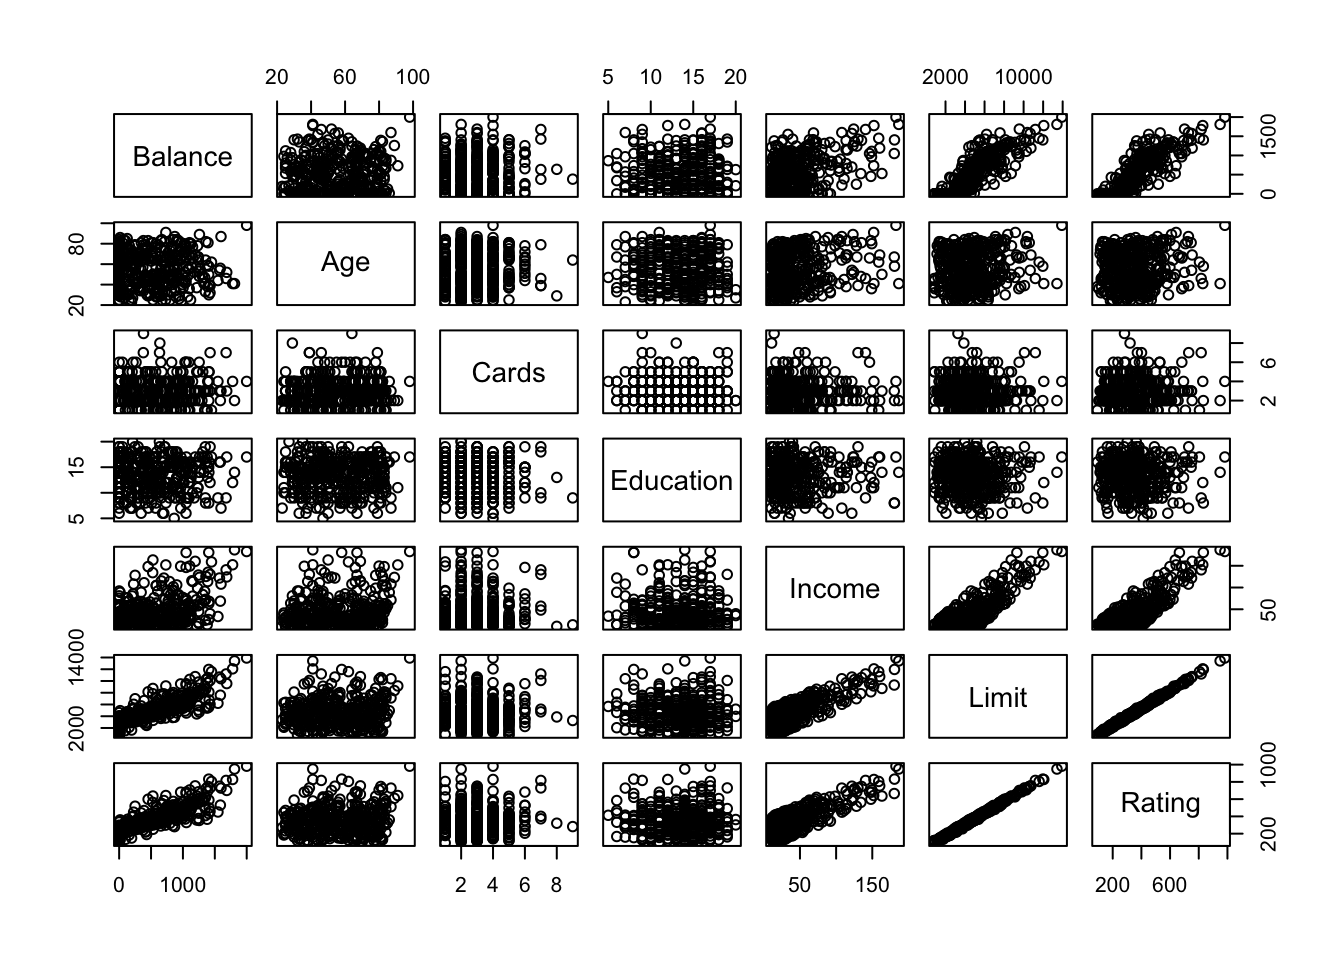
\includegraphics[width=0.5\textwidth,height=\textheight]{credit_card_data.png}
\caption{Credit data figure}
\end{figure}

\hypertarget{recommended-exercise-3}{%
\section{Recommended exercise 3}\label{recommended-exercise-3}}

\begin{enumerate}
\def\labelenumi{\arabic{enumi}.}
\tightlist
\item
  For the Credit Dataset, pick the best model using Best Subset
  Selection according to \(C_p\), \(BIC\) and Adjusted \(R^2\)

  \begin{itemize}
  \tightlist
  \item
    Hint: Use the \texttt{regsubsets()} of the \texttt{leaps} library,
    similar to what was done in Lab 1 of the book.
  \end{itemize}
\item
  For the Credit Dataset, pick the best model using Best Subset
  Selection according to a \(10\)-fold CV

  \begin{itemize}
  \tightlist
  \item
    Hint: Use the output obtained in the previous step and build your
    own CV function to pick the best model.
  \end{itemize}
\item
  Compare the result obtained in Step 1 and Step 2.
\end{enumerate}

\hypertarget{recommended-exercise-4}{%
\section{Recommended exercise 4}\label{recommended-exercise-4}}

\begin{enumerate}
\def\labelenumi{\arabic{enumi}.}
\tightlist
\item
  Select the best model for the Credit Data using Forward, Backward and
  Hybrid (sequential replacement) Stepwise Selection.

  \begin{itemize}
  \tightlist
  \item
    Hint: Use the \texttt{regsubsets()} of the \texttt{leaps} library
  \end{itemize}
\item
  Compare with the results obtained with Best Subset Selection.
\end{enumerate}

\hypertarget{recommended-exercise-5}{%
\section{Recommended exercise 5}\label{recommended-exercise-5}}

\begin{enumerate}
\def\labelenumi{\arabic{enumi}.}
\tightlist
\item
  Apply Ridge regression to the Credit Dataset.
\item
  Compare the results with the standard linear regression.
\end{enumerate}

\hypertarget{recommended-exercise-6}{%
\section{Recommended exercise 6}\label{recommended-exercise-6}}

\begin{enumerate}
\def\labelenumi{\arabic{enumi}.}
\tightlist
\item
  Apply Lasso regression to the Credit Dataset.
\item
  Compare the results with the standard linear regression and the Ridge
  regression.
\end{enumerate}

\hypertarget{recommended-exercise-7}{%
\section{Recommended exercise 7}\label{recommended-exercise-7}}

How many principal components should we use for the Credit Dataset?
Justify.

\hypertarget{recommended-exercise-8}{%
\section{Recommended exercise 8}\label{recommended-exercise-8}}

Apply PCR on the Credit dataset and compare the results with the
previous methods used in this module.

\hypertarget{recommended-exercise-9}{%
\section{Recommended exercise 9}\label{recommended-exercise-9}}

Apply PLS on the Credit dataset and compare the results with the
previous methods used in this module.

\end{document}
